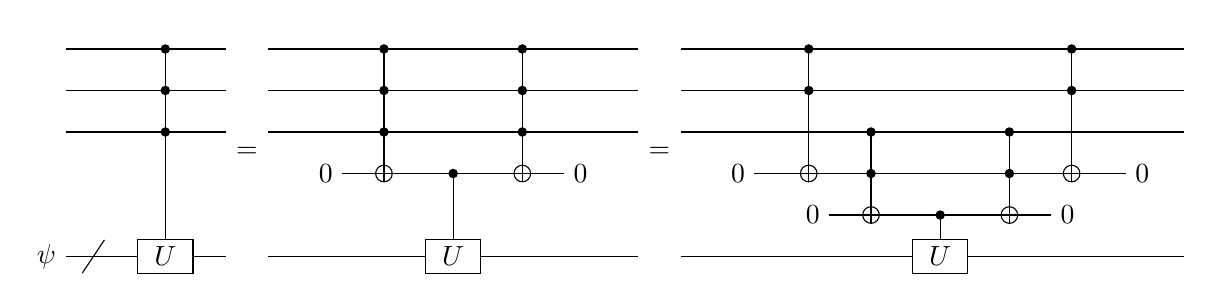
\begin{tikzpicture}[scale=1.000000,x=1pt,y=1pt]
\filldraw[color=white] (0.000000, -7.500000) rectangle (404.000000, 82.500000);
% Drawing wires
% Line 1: 0 W
\draw[color=black] (0.000000,75.000000) -- (404.000000,75.000000);
% Line 2: 1 W
\draw[color=black] (0.000000,60.000000) -- (404.000000,60.000000);
% Line 3: 2 W
\draw[color=black] (0.000000,45.000000) -- (404.000000,45.000000);
% Line 4: c0 W 0 0 0 0
\draw[color=black] (92.500000,30.000000) -- (187.500000,30.000000);
\draw[color=black] (241.500000,30.000000) -- (390.500000,30.000000);
% Line 5: c1 W 0 0
\draw[color=black] (268.500000,15.000000) -- (363.500000,15.000000);
% Line 6: sys W \psi
\draw[color=black] (0.000000,0.000000) -- (404.000000,0.000000);
\draw[color=black] (0.000000,0.000000) node[left] {$\psi$};
% Done with wires; drawing gates
% Line 8: sys /
\draw (6.000000, -6.000000) -- (14.000000, 6.000000);
% Line 10: sys G width=20 $U$ 0 1 2
\draw (36.000000,75.000000) -- (36.000000,0.000000);
\begin{scope}
\draw[fill=white] (36.000000, -0.000000) +(-45.000000:14.142136pt and 8.485281pt) -- +(45.000000:14.142136pt and 8.485281pt) -- +(135.000000:14.142136pt and 8.485281pt) -- +(225.000000:14.142136pt and 8.485281pt) -- cycle;
\clip (36.000000, -0.000000) +(-45.000000:14.142136pt and 8.485281pt) -- +(45.000000:14.142136pt and 8.485281pt) -- +(135.000000:14.142136pt and 8.485281pt) -- +(225.000000:14.142136pt and 8.485281pt) -- cycle;
\draw (36.000000, -0.000000) node {$U$};
\end{scope}
\filldraw (36.000000, 75.000000) circle(1.500000pt);
\filldraw (36.000000, 60.000000) circle(1.500000pt);
\filldraw (36.000000, 45.000000) circle(1.500000pt);
% Line 12: =
\draw[fill=white,color=white] (58.000000, -6.000000) rectangle (73.000000, 81.000000);
\draw (65.500000, 37.500000) node {$=$};
% Line 14: c0 START
\draw[color=black] (100.000000,30.000000) node[fill=white,left,minimum height=15.000000pt,minimum width=15.000000pt,inner sep=0pt] {\phantom{$0$}};
\draw[color=black] (100.000000,30.000000) node[left] {$0$};
% Line 15: 0 1 2 +c0
\draw (115.000000,75.000000) -- (115.000000,30.000000);
\filldraw (115.000000, 75.000000) circle(1.500000pt);
\filldraw (115.000000, 60.000000) circle(1.500000pt);
\filldraw (115.000000, 45.000000) circle(1.500000pt);
\begin{scope}
\draw[fill=white] (115.000000, 30.000000) circle(3.000000pt);
\clip (115.000000, 30.000000) circle(3.000000pt);
\draw (112.000000, 30.000000) -- (118.000000, 30.000000);
\draw (115.000000, 27.000000) -- (115.000000, 33.000000);
\end{scope}
% Line 16: sys G width=20 $U$ c0
\draw (140.000000,30.000000) -- (140.000000,0.000000);
\begin{scope}
\draw[fill=white] (140.000000, -0.000000) +(-45.000000:14.142136pt and 8.485281pt) -- +(45.000000:14.142136pt and 8.485281pt) -- +(135.000000:14.142136pt and 8.485281pt) -- +(225.000000:14.142136pt and 8.485281pt) -- cycle;
\clip (140.000000, -0.000000) +(-45.000000:14.142136pt and 8.485281pt) -- +(45.000000:14.142136pt and 8.485281pt) -- +(135.000000:14.142136pt and 8.485281pt) -- +(225.000000:14.142136pt and 8.485281pt) -- cycle;
\draw (140.000000, -0.000000) node {$U$};
\end{scope}
\filldraw (140.000000, 30.000000) circle(1.500000pt);
% Line 17: 0 1 2 +c0
\draw (165.000000,75.000000) -- (165.000000,30.000000);
\filldraw (165.000000, 75.000000) circle(1.500000pt);
\filldraw (165.000000, 60.000000) circle(1.500000pt);
\filldraw (165.000000, 45.000000) circle(1.500000pt);
\begin{scope}
\draw[fill=white] (165.000000, 30.000000) circle(3.000000pt);
\clip (165.000000, 30.000000) circle(3.000000pt);
\draw (162.000000, 30.000000) -- (168.000000, 30.000000);
\draw (165.000000, 27.000000) -- (165.000000, 33.000000);
\end{scope}
% Line 18: c0 END
\draw[color=black] (180.000000,30.000000) node[fill=white,right,minimum height=15.000000pt,minimum width=15.000000pt,inner sep=0pt] {\phantom{$0$}};
\draw[color=black] (180.000000,30.000000) node[right] {$0$};
% Line 20: =
\draw[fill=white,color=white] (207.000000, -6.000000) rectangle (222.000000, 81.000000);
\draw (214.500000, 37.500000) node {$=$};
% Line 22: c0 START
\draw[color=black] (249.000000,30.000000) node[fill=white,left,minimum height=15.000000pt,minimum width=15.000000pt,inner sep=0pt] {\phantom{$0$}};
\draw[color=black] (249.000000,30.000000) node[left] {$0$};
% Line 23: 0 1 +c0
\draw (268.500000,75.000000) -- (268.500000,30.000000);
\filldraw (268.500000, 75.000000) circle(1.500000pt);
\filldraw (268.500000, 60.000000) circle(1.500000pt);
\begin{scope}
\draw[fill=white] (268.500000, 30.000000) circle(3.000000pt);
\clip (268.500000, 30.000000) circle(3.000000pt);
\draw (265.500000, 30.000000) -- (271.500000, 30.000000);
\draw (268.500000, 27.000000) -- (268.500000, 33.000000);
\end{scope}
% Line 24: c1 START
\draw[color=black] (276.000000,15.000000) node[fill=white,left,minimum height=15.000000pt,minimum width=15.000000pt,inner sep=0pt] {\phantom{$0$}};
\draw[color=black] (276.000000,15.000000) node[left] {$0$};
% Line 25: c0 2 +c1
\draw (291.000000,45.000000) -- (291.000000,15.000000);
\filldraw (291.000000, 30.000000) circle(1.500000pt);
\filldraw (291.000000, 45.000000) circle(1.500000pt);
\begin{scope}
\draw[fill=white] (291.000000, 15.000000) circle(3.000000pt);
\clip (291.000000, 15.000000) circle(3.000000pt);
\draw (288.000000, 15.000000) -- (294.000000, 15.000000);
\draw (291.000000, 12.000000) -- (291.000000, 18.000000);
\end{scope}
% Line 26: sys G width=20 $U$ c1
\draw (316.000000,15.000000) -- (316.000000,0.000000);
\begin{scope}
\draw[fill=white] (316.000000, -0.000000) +(-45.000000:14.142136pt and 8.485281pt) -- +(45.000000:14.142136pt and 8.485281pt) -- +(135.000000:14.142136pt and 8.485281pt) -- +(225.000000:14.142136pt and 8.485281pt) -- cycle;
\clip (316.000000, -0.000000) +(-45.000000:14.142136pt and 8.485281pt) -- +(45.000000:14.142136pt and 8.485281pt) -- +(135.000000:14.142136pt and 8.485281pt) -- +(225.000000:14.142136pt and 8.485281pt) -- cycle;
\draw (316.000000, -0.000000) node {$U$};
\end{scope}
\filldraw (316.000000, 15.000000) circle(1.500000pt);
% Line 27: c0 2 +c1
\draw (341.000000,45.000000) -- (341.000000,15.000000);
\filldraw (341.000000, 30.000000) circle(1.500000pt);
\filldraw (341.000000, 45.000000) circle(1.500000pt);
\begin{scope}
\draw[fill=white] (341.000000, 15.000000) circle(3.000000pt);
\clip (341.000000, 15.000000) circle(3.000000pt);
\draw (338.000000, 15.000000) -- (344.000000, 15.000000);
\draw (341.000000, 12.000000) -- (341.000000, 18.000000);
\end{scope}
% Line 28: c1 END
\draw[color=black] (356.000000,15.000000) node[fill=white,right,minimum height=15.000000pt,minimum width=15.000000pt,inner sep=0pt] {\phantom{$0$}};
\draw[color=black] (356.000000,15.000000) node[right] {$0$};
% Line 29: 0 1 +c0
\draw (363.500000,75.000000) -- (363.500000,30.000000);
\filldraw (363.500000, 75.000000) circle(1.500000pt);
\filldraw (363.500000, 60.000000) circle(1.500000pt);
\begin{scope}
\draw[fill=white] (363.500000, 30.000000) circle(3.000000pt);
\clip (363.500000, 30.000000) circle(3.000000pt);
\draw (360.500000, 30.000000) -- (366.500000, 30.000000);
\draw (363.500000, 27.000000) -- (363.500000, 33.000000);
\end{scope}
% Line 30: c0 END
\draw[color=black] (383.000000,30.000000) node[fill=white,right,minimum height=15.000000pt,minimum width=15.000000pt,inner sep=0pt] {\phantom{$0$}};
\draw[color=black] (383.000000,30.000000) node[right] {$0$};
% Done with gates; drawing ending labels
% Done with ending labels; drawing cut lines and comments
% Done with comments
\end{tikzpicture}
